\documentclass{article}

\usepackage{amsmath, amsthm, amssymb, latexsym, amsfonts}
\usepackage{comment, enumerate, mathrsfs, stmaryrd, hyperref}
\usepackage{tikz}
\usepackage{xcolor}
\usepackage{graphicx}
\usepackage{titlesec}
\usepackage{booktabs}
\usepackage{graphicx}
\usepackage{tabularx}
\usepackage{blindtext}
\usepackage[a4paper, total={7in, 9in}]{geometry}

\begin{document}

\begin{titlepage}
    \begin{center}
        \vspace*{0.6cm}
            
        \Huge
        \textbf{Do you like Texas hold 'em}
            
        \vspace{0.5cm}
        \LARGE
        STAT230 Real World Assignment 2024W
            
        \vspace{1.5cm}
            
        \textbf{Eason Li, Johnson Ji}
            
        \vspace{3.6cm}
        
        \begin{center}
            
\includegraphics[width = 0.4\textwidth]{UofLoo.png}
        \end{center}

        \vspace{0.4cm}
            
        \Large
        Falculty of Math \\
        University of Waterloo \\
        Canada \\
        April 8, 2024
    \end{center}
\end{titlepage}

\newpage

\begin{center}
    \textcolor{blue}{
        In this report, we consider the case a player uses the best 
        five-card poker hand out of seven cards.
    }
\end{center}

For a 7-card hand to contain a Royal Flush, i.e.
\begin{center}
    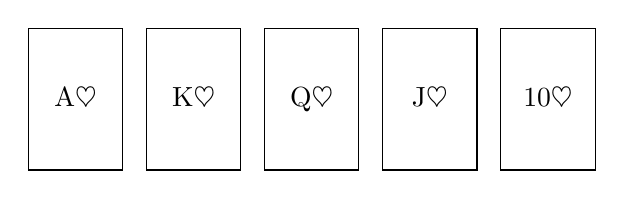
\begin{tikzpicture}
        \foreach \rank/\suit/\x in {A/\(\heartsuit\)/0, K/\(\heartsuit\)/1.5, Q/\(\heartsuit\)/3, J/\(\heartsuit\)/4.5, 10/\(\heartsuit\)/6} {
        % Draw the card
        \draw (\x,0) rectangle ++(1.2,1.8);
        % Add the rank and suit
        \node at (\x+0.6,0.9) {\rank\suit};
        }
    \end{tikzpicture}
\end{center}
it must contain the specific set of 5 cards 
(Ace, King, Queen, Jack, 10 of the same suit), 
with the other 2 cards being any of the remaining 47 cards in the deck. 
Therefore, the probability of getting a Royal Flush in a group of seven 
cards can be evaluated as 
\[
P(\text{Royal Flush in 7-card poker}) = \frac{4 \times C(47, 2)}{C(52, 7)}
\]
With the similar idea, we can get discover the following probabilities:
\begin{table}[ht]
    \centering
    \caption{Probabilities of Being Dealt Specific Hands in Texas Hold'em Poker (7 cards)}
    \label{tab:poker_hands}
    \begin{tabularx}{\textwidth}{@{}Xc@{}} % Using tabularx to make the table span the text width
    \toprule
    Hand Rank                  & Absolute frequency (\%) \\ \midrule
    Royal Flush                & $\displaystyle \frac{4 \times C(47, 2)}{C(52, 7)}$       \\
    \\
    Straight Flush (non-Royal) & 0.00139          \\
    Four of a Kind             & 0.0240           \\
    Full House                 & 0.1441           \\
    Flush                      & 0.197            \\
    Straight                   & 0.392            \\
    Three of a Kind            & 2.112            \\
    Two Pair                   & 4.753            \\
    One Pair                   & 42.256           \\
    High Card                  & 50.117           \\ \bottomrule
    \end{tabularx}
\end{table}







\end{document}
